\chapter{M\'etodo Matricial de Ursin para Solu\c{c}\~ao de EDP's}

\section{Introdu\c{c}\~ao}
Este cap\'itulo trata da utiliza\c{c}\~ao de um m\'etodo matricial para estudar a propaga\c{c}\~ao de ondas em subsuperf\'icie terrestre, conforme estruturado em \cite{Ursin-1983}. Gra\c{c}as a similaridade matem\'atica entre sistemas de EDP's eletromagn\'eticas e sistemas de EDP's el\'asticas, podemos dar um desenvolvimento unificado para esses sistemas. Utilizamos um conjunto de transformadas (Fourier, Laplace e Bessel) para escrever cada um desses sistemas de EDP's numa forma matricial, em fun\c{c}\~ao apenas da profundidade, composta por $2n$ equa\c{c}\~oes diferenciais ordin\'arias. Os coeficientes desse sistema de EDO's podem ser reunidos numa matriz $A$ de dimens\~ao $2n\times 2n$, a qual pode ser particionada em quatro submatrizes de dimens\~ao $n\times n$, e \'e usada como o ponto de partida para o estudo da propaga\c{c}\~ao de ondas em subsuperf\'icie.  

As propriedades de simetria da matriz $A$ nos permitem separar o campo de ondas em ascendentes e descendentes atrav\'es de uma decomposi\c{c}\~ao em autovetores. Essas propriedades nos permitem tamb\'em deduzir caracter\'isticas invariantes da propaga\c{c}\~ao, onde uma dessas caracter\'isticas \'e v\'alida apenas para meios de baixa dissipa\c{c}\~ao de ondas e correspondem \`a conserva\c{c}\~ao de energia. A matriz de propaga\c{c}\~ao de ondas pode ser computada para camadas homog\^eneas ou n\~ao, atrav\'es de um m\'etodo relativamente simples. Dado o vetor de ondas na camada superficial, podemos calcular seu valor para qualquer camada usando a matriz de propaga\c{c}\~ao.

A propaga\c{c}\~ao de ondas em meios estratificados produz fen\^omenos de transmiss\~ao e reflex\~ao de ondas. Dadas as defini\c{c}\~oes das matrizes de transmiss\~ao e reflex\~ao, podemos relacion\'a-las com a matriz de propaga\c{c}\~ao, bem como deduzir propriedades de simetrias para essas matrizes atrav\'es das caracter\'isticas invariantes da propaga\c{c}\~ao. Podemos ainda deduzir as matrizes de transmiss\~ao e reflex\~ao modificadas para pilha de camadas limitadas superiormente por uma superf\'icie livre.

\section{Sistema de EDP's do Efeito Magnetoel\'astico}

Segundo \cite{eringen_1963}, o acoplamento entre ondas eletromagn\'eticas e el\'asticas se propagando no subsolo caracteriza o efeito magnetoel\'astico, e esse acoplamento pode ser modelado matematicamente atrav\'es de um sistema de equa\c{c}\~oes diferencias parciais. Conforme minha monografia, podemos aplicar uma s\'erie de hip\'oteses que visam simplificar e linearizar essas EDP's de forma que as mesmas possam receber um tratamento matem\'atico adequado no sentido de se obter numericamente os valores dos campos eletromagn\'eticos e el\'asticos envolvidos no sistema. Desta forma, vamos utilizar o m\'etodo matricial encontrado em \cite{Ursin-1983} na solu\c{c}\~ao do seguinte sistema de EDP's da magnetoelasticidade
\begin{align*}
\nabla\times\mathbf{\widehat{E}}&=i\,\omega\,\mu_0\mathbf{\widehat{H}}\\\\
\nabla\times\mathbf{\widehat{H}}&=(\sigma-i\,\epsilon\,\omega)\,\mathbf{\widehat{E}}+\mathbf{\widehat{v}}\times\sigma\mu_0\mathbf{H}^0\\\\
-i\,\omega\rho\,\mathbf{\widehat{v}}&=\nabla\cdot\widehat{\tau} + \mathbf{\widehat{F}}\\\\
\widehat{\tau}&=\lambda\,\nabla\cdot\mathbf{\widehat{u}}\cdot\,I + \mu\,(\nabla\,\mathbf{\widehat{u}}+\nabla\mathbf{\widehat{u}}^\top)\\\\
\nabla\cdot\mathbf{\widehat{H}}&=0.
\end{align*}
Onde, o dom\'inio da frequ\^encia \'e indicado pelo nota\c{c}\~ao $\widehat{\,.\,}$, e 
\begin{itemize}
\item $\mathbf{\widehat{E}}$ \'e o campo el\'etrico,
\item $\mathbf{\widehat{B}}$ \'e o campo magn\'etico,
\item $\mathbf{\widehat{D}}$ \'e o campo de densidade de fluxo el\'etrico,
\item $\mathbf{\widehat{H}}$ \'e o campo magn\'etico auxiliar,
\item $\tau$ \'e o tensor de tens\~oes,
\item $\mathbf{\widehat{u}}$ \'e o deslocamento do meio,
\item $\mathbf{\widehat{v}}$ \'e a velocidade de deslocamento do meio,
\item $\mathbf{\widehat{F}}$ \'e uma for\c{c}a aplicada ao meio,
\item $\mathbf{H}^0$ \'e campo geomagn\'etico,
\item $i$ \'e um n\'umero complexo,
\item $\omega$ \'e a frequ\^encia temporal,
\item $\mu_0$ \'e a permeabilidade magn\'etica no v\'acuo,
\item $\sigma$ \'e a condutividade do meio,
\item $\epsilon$ \'e a permissividade el\'etrica do meio,
\item $\rho$ \'e a densidade do meio,
\item $\lambda$ e $\mu$ s\~ao par\^ametros de Lam\`e.
\end{itemize}
Vamos definir $\sigma^*=(\sigma-i\,\epsilon\,\omega)$. No subsolo, por conta do regime quasi-estacion\'ario, $(\sigma>>\epsilon\,\omega)$  e  temos $\sigma^*=\sigma$. No ar, a condutividade \'e zero e a permeabilidade el\'etrica \'e pr\'oxima a do v\'acuo $\epsilon_0$, assim temos $\sigma^*=-i\,\epsilon_0\omega$.

\section{Escrevendo as Equa\c{c}\~oes na Forma Matricial}

Sendo $\mathbf{x}=(x,y,z)^{\top}$ o espa\c{c}o $\mathbb{R}^3$ e aplicando as tranformadas de Fourier direta e inversa na forma
\begin{align*}
F(\omega,k_1,k_2,z) &= \iiint_{-\infty}^{\infty}f(t,x,y,z)\,e^{i\omega t-ik_1x-ik_2y}dt\,dxdy\\\\
f(t,x,y,z) &= \left(\frac{1}{2\,\pi}\right)^3\,\iiint_{-\infty}^{\infty}F(\omega,k_1,k_2,z)\,e^{-i\omega t+ik_1x+ik_2y}d\omega\,dk_1dk_2\,,
\end{align*}
podemos escrever um conjunto de EDP's que descevem a propaga\c{c}\~ao de ondas sismomagn\'eticas em camadas horizontais da subsuperf\'icie terrestre somente em fun\c{c}\~ao da profundidade $z$. 

A t\'itulo de exemplo, tanto as EDP's de Maxwell para o eletromagnetismo
\begin{align}\label{eq.faraday_ampere}\nonumber
\nabla\times\mathbf{E}&=-\frac{\partial}{\partial t}\mathbf{B}\\\\\nonumber
\nabla\times\mathbf{H}&=\sigma\mathbf{E}+\frac{\partial}{\partial t}\mathbf{D}+\mathbf{G}\,,
\end{align}
como as EDP's el\'asticas
\begin{align}\label{eq.cauchy_hooke}\nonumber
\rho\frac{\partial^2 \mathbf{U}}{\partial t^2}&=\nabla\cdot\tau+\mathbf{F}\\\\\nonumber
\tau&=\lambda\nabla\cdot \mathbf{U}\cdot I + \mu(\nabla \mathbf{U}+\nabla \mathbf{U}^*)\,,
\end{align}
podem ser escritas no formato matricial apresentado por Ursin, ou seja, cada um desses sistemas, isoladamente, pode ser escrito na forma 
\begin{align}\label{eq.matricial}
\frac{\partial\,\mathbf{B}}{\partial\,z} &= \pm\,i\,\omega\,A\,\mathbf{B} = \pm\,i\,\omega\,
\begin{bmatrix}
0&A_1\\
A_2&0
\end{bmatrix}\,
\begin{bmatrix}
\mathbf{B_1}\\
\mathbf{B_2}	
\end{bmatrix}\,,
\end{align}
onde o vetor $\mathbf{B}$ representa uma onda qualquer e n\~ao o campo magn\'etico dado em \ref{eq.faraday_ampere}.

A equação \ref{eq.matricial} tem as seguintes caracter\'isticas:
\begin{itemize}
\item $A_{2\,n\times2\,n}$ \'e uma matriz que pode ser particionada em quatro submatrizes $n\times n$, com submatrizes de zeros na diagonal principal e submatrizes sim\'etricas $A_1$ e $A_2$ na diagonal secund\'aria. As componentes de $A_1$ e $A_2$ s\~ao fun\c{c}\~oes dos par\^ametros das EDP's \ref{eq.faraday_ampere} e \ref{eq.cauchy_hooke}, s\~ao fun\c{c}\~oes tamb\'em de $z$ e do vetor real de retardamento $\mathbf{p}=\frac{\mathbf{k}}{\omega}$. Para meios de baixa dissipa\c{c}\~ao das ondas, as matrizes $A_1$ e $A_2$ s\~ao reais; 
\item O vetor de onda $\mathbf{B}$ tem dimens\~ao $2n\times1$ e \'e particionado em dois vetores $\mathbf{B}_1$ e $\mathbf{B}_2$ com dimens\~ao $n\times1$ . As componentes do vetor de onda s\~ao escolhidas de forma que $\mathbf{B}$ seja cont\'inuo atrav\'es das fronteiras entre duas camadas;
\item  Para ondas el\'asticas, metade das componentes de $\mathbf{B}$ s\~ao zeros na superf\'icie livre, ou seja, existe uma matriz de permuta\c{c}\~ao $T_{2n\times2n}$ onde $T^{-1}=T^\top$ e tal que
\begin{equation*}
\begin{bmatrix}
\mathbf{V}_1(\mathbf{0})\\
\mathbf{0}
\end{bmatrix}
=T\,\mathbf{B}\quad\text{quando}\quad z = 0\,;
\end{equation*}
\item As componentes do vetor de onda $\mathbf{B}$ s\~ao escolhidas de forma que o fluxo de energia na dire\c{c}\~ao $z$ seja dado por
\begin{equation*}
J=-\frac{1}{4}(\mathbf{B}_1^H\mathbf{B}_2+\mathbf{B}_2^H\mathbf{B}_1)=-\frac{1}{4}\mathbf{B}^H\,M\, \mathbf{B}\,,
\end{equation*}
onde $H$ denota complexo conjugado transposto,
\begin{equation*}
M=
\begin{bmatrix}
0_{n\times n}&I\\
I&0_{n\times n}
\end{bmatrix}
\end{equation*}
e $I$ \'e uma matriz identidade $n\times n$.
\end{itemize}

Os m\'etodos a seguir s\~ao aplicados em equa\c{c}\~oes escritas no formato matricial \ref{eq.matricial}, com ondas se propagando numa pilha de camadas homog\^eneas e assumimos que os par\^ametros das equa\c{c}\~oes s\~ao fun\c{c}\~oes cont\'inuas no interior de cada camada que dependem apenas da profundidade $z$. O modelo inclui pilha de camadas homog\^eneas com par\^ametros constantes por camada e consideramos o eixo $z$ como sendo positivo no sentido descendente.   

\section{Decomposi\c{c}\~ao em Ondas Ascendentes e Descentes}

Para realizar a decomposi\c{c}\~ao do vetor $\mathbf{B}$ em ondas ascendentes e descendentes aplicamos uma diagonaliza\c{c}\~ao em autovalores na matriz $A$ na forma
\begin{equation}\label{eq.diagonalizacao}
A=L\,\Lambda_1L^{-1}\,,
\end{equation}
onde $\Lambda_1$ \'e a matriz diagonal dos autovalores $\lambda_i$ para $i=1,2,...,n$, e $L$ \'e a matriz dos autovetores correspondentes,
\begin{equation}\label{eq.Lambda_1}
\Lambda_1=
\begin{bmatrix}
\Lambda&0\\
0&-\Lambda
\end{bmatrix}\,.
\end{equation} 
A defini\c{c}\~ao de autovalores e autovetores \'e dada por
\begin{equation}\label{eq.sist_autovalores}
\begin{bmatrix}
0&A_1\\
A_2&0
\end{bmatrix}
\begin{bmatrix}
\mathbf{L_1}\\
\mathbf{L_2}
\end{bmatrix}
=
\lambda\,
\begin{bmatrix}
\mathbf{L_1}\\
\mathbf{L_2}
\end{bmatrix}
\end{equation}
e aplicando o procedimento
\begin{equation*}
\begin{bmatrix}
0&A_1\\
A_2&0
\end{bmatrix}
\begin{bmatrix}
0&A_1\\
A_2&0
\end{bmatrix}
\begin{bmatrix}
\mathbf{L_1}\\
\mathbf{L_2}
\end{bmatrix}
=
\lambda\,\lambda\,
\begin{bmatrix}
\mathbf{L_1}\\
\mathbf{L_2}
\end{bmatrix}\,,
\end{equation*}
podemos separar o sitema \ref{eq.sist_autovalores} de dimens\~ao $2n$ em dois sistemas de dimens\~ao n
\begin{align*}
A_1A_2\mathbf{L_1}&=\lambda^2\mathbf{L_1}\\
A_2A_1\mathbf{L_2}&=\lambda^2\mathbf{L_2}\,,
\end{align*}
onde $\mathbf{L}_i$ s\~ao os vetores que, concatenados dois a dois, formam os autovetores que comp\~oem $L$.
Assim, podemos dividir a diagonaliza\c{c}\~ao dada em \ref{eq.diagonalizacao} em duas diagonaliza\c{c}\~oes de dimens\~ao $n$
\begin{align}\label{eq.subdiagonalizacao}\nonumber
A_1A_2&=L_1\Lambda^2L_1^{-1}\\\quad\\\nonumber
A_2A_1&=L_2\Lambda^2L_2^{-1}\,,
\end{align}
onde $L_i$ s\~ao submatrizes da matriz $L$ e cont\^em os autovetores $\mathbf{L}_i$.



Definindo a matriz 
\begin{equation}\label{eq.L}
L=\frac{1}{\sqrt{2}}
\begin{bmatrix}
L_1&L_1\\
L_2&-L_2
\end{bmatrix}
\end{equation}
e sua inversa
\begin{equation}\label{eq.L_inversa}
L^{-1}=\frac{1}{\sqrt{2}}
\begin{bmatrix}
L_1^{-1}&L_2^{-1}\\
L_1^{-1}&-L_2^{-1}
\end{bmatrix}\,,
\end{equation}
podemos substitu\'i-las na equa\c{c}\~ao \ref{eq.diagonalizacao} e verificar que 
\begin{align}\label{eq.definicao_A1_A2}\nonumber
A_1&=L_1\Lambda\,L_2^{-1}\\\quad\\\nonumber
A_2&=L_2\Lambda\,L_1^{-1}\,,
\end{align}
e podemos verificar ainda que essas defini\c{c}\~oes para $A_1$ e $A_2$ satisfazem tamb\'em as equa\c{c}\~oes \ref{eq.subdiagonalizacao}.

Pelas caracter\'isticas da equa\c{c}\~ao \ref{eq.matricial} sabemos que as matrizes $A_1$ e $A_2$ s\~ao sim\'etricas e podem ser escritas como
\begin{align*}
A_1&=L_2^{-\top}\Lambda\,L_1^\top\\
A_2&=L_1^{-\top}\Lambda\,L_2^\top\,,
\end{align*}
as quais substitu\'idas nas equa\c{c}\~oes \ref{eq.subdiagonalizacao} lucramos
\begin{equation*}
A_1A_2=L_1\Lambda^2L_1^{-1}=L_2^{-\top}\Lambda^2L_2^\top\,,
\end{equation*}
e conclu\'imos que, a menos da escala dos autovetores,
\begin{equation*}
L_1=L_2^{-\top}\,.
\end{equation*}
Substituindo a \'ultima igualdade na defini\c{c}\~ao \ref{eq.definicao_A1_A2} temos
\begin{equation*}
A_i=L_i\Lambda\,L_i^{\top}\qquad\text{para}\qquad i=1\,\text{e}\,2\,,
\end{equation*}
e substituindo em \ref{eq.L_inversa}, temos
\begin{equation}\label{eq.L_inversa_2}
L^{-1}=\frac{1}{\sqrt{2}}
\begin{bmatrix}
L_2^{\top}&L_1^{\top}\\
L_2^{\top}&-L_1^{\top}
\end{bmatrix}\,.
\end{equation}

Escrevendo o vetor de ondas na forma
\begin{equation}\label{eq.transformacao_B}
\mathbf{B}=L\,\mathbf{W}\,,
\end{equation}
aplicando a derivada parcial em rela\c{c}\~ao a $z$, e substituindo as equa\c{c}\~oes \ref{eq.matricial} e \ref{eq.diagonalizacao}, obtemos
\begin{equation}\label{eq.derivada_W}
\frac{\partial\mathbf{W}}{\partial\,z}=\left[\pm i\omega\,\Lambda_1-L^{-1}\frac{\partial\,L}{\partial\,z}\right]\,\mathbf{W}\,.
\end{equation}
Para a propaga\c{c}\~ao de ondas em camadas homog\^eneas, os coeficientes das EDP's originais s\~ao constantes por camada e esses coeficientes comp\~oem a matriz $A$ diagonalizada pela matriz $L$. Assim, para meios homog\^eneos, a \'ultima equa\c{c}\~ao pode ser reduzida a
\begin{equation*}
\frac{\partial\mathbf{W}}{\partial\,z}=\pm i\omega\,\Lambda_1\mathbf{W}\,.
\end{equation*}
Representamos o vetor $\mathbf{W}$ como
\begin{equation*}
\mathbf{W}=
\begin{bmatrix}
\mathbf{U}\\
\mathbf{D}
\end{bmatrix}\,,
\end{equation*}
onde $\mathbf{U}$ e $\mathbf{D}$ s\~ao vetores que representam ondas ascendentes e descendentes, respectivamente, desde que a parte real de $\pm i\omega\lambda_i$ seja n\~ao negativa para $i=1,2,...,n$.

Substiutindo as equa\c{c}\~oes \ref{eq.L} e \ref{eq.L_inversa_2} na equa\c{c}\~ao \ref{eq.derivada_W} e efetuando as multiplica\c{c}\~oes matriciais obtemos
\begin{align}\label{eq.Up_Down}\nonumber
\frac{\partial\mathbf{U}}{\partial z}&=\pm i\omega\,\Lambda\,\mathbf{U}+F\,\mathbf{U}+G\,\mathbf{D}\\\quad\\\nonumber
\frac{\partial\mathbf{D}}{\partial z}&=\pm i\omega\,\Lambda\,\mathbf{D}+F\,\mathbf{D}+G\,\mathbf{U}
\end{align}
onde as matrizes $F$ e $G$ s\~ao, respectivamente,
\begin{align*}
F&=-\frac{1}{2}\left[L_2^\top\frac{\partial L_1}{\partial z}+L_1^\top\frac{\partial L_2}{\partial z}\right]\\\quad\\
G&=-\frac{1}{2}\left[L_2^\top\frac{\partial L_1}{\partial z}-L_1^\top\frac{\partial L_2}{\partial z}\right]\,.
\end{align*}
Substituindo $F$ e $G$ nas express\~oes
\begin{equation*}
-2(F+F^\top)\quad\text{e}\quad-2(G-G^\top)\,,
\end{equation*}
verificamos que ambas as express\~oes s\~ao nulas e, consequentemente,
\begin{equation*}
F=-F^\top\quad\text{e}\quad G=G^\top\,.
\end{equation*}
Para propaga\c{c}\~ao em camadas homog\^eneas e isotr\'opicas, podemos  negligenciar as \'ultimas parcelas das equa\c{c}\~oes \ref{eq.Up_Down} e temos a express\~ao final para ondas ascendentes e descendentes, respectivamente,
\begin{align}\label{eq.Up_Down_2}\nonumber
\frac{\partial\mathbf{U}}{\partial z}&=\pm i\omega\,\Lambda\,\mathbf{U}\\\quad\\\nonumber
\frac{\partial\mathbf{D}}{\partial z}&=\pm i\omega\,\Lambda\,\mathbf{D}\,.
\end{align}


\section{Matriz de Propaga\c{c}\~ao}

Podemos utilizar a equa\c{c}\~ao \ref{eq.matricial} para calcular o valor do vetor de ondas numa profundidade qualquer $\mathbf{B}_z$, desde que saibamos o valor do vetor na superf\'icie $\mathbf{B}_0$ e mantendo a frequ\^encia e o vetor de retardamento constantes. Para ondas descendentes, a \textit{matriz de propaga\c{c}\~ao} \'e dada pela solu\c{c}\~ao da equa\c{c}\~ao 
\begin{equation}\label{eq.matriz_propagacao}
\frac{\partial P(z,z_0)}{\partial z}=\pm i\omega\,A(z)\,P(z,z_0)\,,
\end{equation}
onde $P(z_0,z_0)=I$. Para ondas ascendentes, a matriz de propaga\c{c}\~ao \'e dada por
\begin{equation*}
\frac{\partial P(\zeta,z_N)}{\partial \zeta}=\pm i\omega A(\zeta)\,P(\zeta,z_N)\,,
\end{equation*}
onde $P(z_N,z_N)=I$.

Sabendo o valor de $\mathbf{B}(z_0)$, a solu\c{c}\~ao da equa\c{c}\~ao \ref{eq.matricial} \'e dada por
\begin{equation*}
\mathbf{B}(z)=P(z,z_0)\,\mathbf{B}(z_0)\,,
\end{equation*}
e podemos notar que 
\begin{equation*}
P^{-1}(z_N,z_0)=P(z_0,z_N)\,.
\end{equation*}
As condi\c{c}\~oes de fronteiras preconizam que o vetor de ondas \'e cont\'inuo atrav\'es das interfaces, o que implica que a matriz de propaga\c{c}\~ao tamb\'em se mant\'em cont\'inua na interface entre duas camadas homog\^eneas ou n\~ao.

Considerando a transforma\c{c}\~ao dada pela equa\c{c}\~ao \ref{eq.transformacao_B}, a matriz de propaga\c{c}\~ao para ondas descendentes $Q(z,z_0)$ associada ao vetor $\mathbf{W}$ \'e a solu\c{c}\~ao da equa\c{c}\~ao
\begin{equation}\label{eq.Q_nao_homogenea}
\frac{\partial\,Q(z,z_0)}{\partial z}=
\begin{bmatrix}
\pm i\omega\,\Lambda+F&G\\
G&\pm i\omega\,\Lambda+F
\end{bmatrix}
Q(z,z_0)\,,
\end{equation}
onde $Q(z_0,z_0)=I$.

E, para ondas ascendentes, temos
\begin{equation*}
\frac{\partial\,Q(\zeta,z_N)}{\partial \zeta}=-
\begin{bmatrix}
\pm i\omega\,\Lambda+F&G\\
G&\pm i\omega\,\Lambda+F
\end{bmatrix}
Q(\zeta,z_N)\,,
\end{equation*}
com $Q(z_N,z_N)=I$.

No caso de uma pilha de camadas homog\^eneas com a espessura de uma camada $k$ dada por $\Delta z_k=z_k-z_{k-1}$, onde $z_k$ \'e a profundidade da interface entre a camada $k$ e a camada $k+1$. Nesta condi\c{c}\~ao e usando a equa\c{c}\~ao \ref{eq.diagonalizacao}, a equa\c{c}\~ao da matriz de propaga\c{c}\~ao \ref{eq.matriz_propagacao} pode ser integrada diretamente  
\begin{align*}
P(z,z_0)&=\exp{\pm i\omega\,A(z-z_0)}\\
&=L\,\left[\exp{\pm i\omega\,\Lambda_1(z-z_0)}\right]\,L^{-1}\,.
\end{align*}
Ou, escrevendo em termos matriciais e usando as equa\c{c}\~oes \ref{eq.Lambda_1}, \ref{eq.L} e \ref{eq.L_inversa_2}, temos
\begin{equation*}
P(z,z_0)=
\begin{bmatrix}
L_1\cosh[\pm i\omega\,\Lambda(z-z_0)]L^\top_2&L_1\sinh[\pm i\omega\,\Lambda(z-z_0)]L^\top_1\\
L_2\sinh[\pm i\omega\,\Lambda(z-z_0)]L^\top_2&L_2\cosh[\pm i\omega\,\Lambda(z-z_0)]L^\top_1
\end{bmatrix}\,,
\end{equation*}
onde
\begin{align*}
\cosh[\pm i\omega\,\Lambda(z-z_0)]&=\frac{1}{2}\exp\left[\pm i\omega\,\Lambda(z-z_0)\right]+\frac{1}{2}\exp\left[-\pm i\omega\,\Lambda(z-z_0)\right]\\\quad\\
\sinh[\pm i\omega\,\Lambda(z-z_0)]&=\frac{1}{2}\exp\left[\pm i\omega\,\Lambda(z-z_0)\right]-\frac{1}{2}\exp\left[-\pm i\omega\,\Lambda(z-z_0)\right]\,.
\end{align*}

Integrando a equa\c{c}\~ao \ref{eq.Q_nao_homogenea} e considerando camadas homog\^eneas, a matriz de propaga\c{c}\~ao $Q$ fica
\begin{equation}\label{eq.Q(z,z_0)}
Q(z,z_0)=
\begin{bmatrix}
\exp{\pm i\omega\,\Lambda(z-z_0)}&0\\
0&\exp{\pm i\omega\,\Lambda(z-z_0)}
\end{bmatrix}\,.
\end{equation}

\section{Propriedades Invariantes da Propaga\c{c}\~ao}
As propriedades da matriz $A$ determinam as caracter\'isticas de propaga\c{c}\~ao do vetor de ondas $\mathbf{B}$. Como as matrizes $A_1$ e $A_2$ s\~ao sim\'etricas, podemos verificar que a fun\c{c}\~ao $G$ dada por
\begin{equation*}
G(\mathbf{B},\mathbf{C})=-(\mathbf{B}_1^\top\mathbf{C_2-\mathbf{B}_2^\top\mathbf{C}_1})\,,
\end{equation*}
ou por
\begin{equation*}
G(\mathbf{B},\mathbf{C})=-\mathbf{B}^\top N\,\mathbf{C}\qquad\text{com}\qquad N=
\begin{bmatrix}
0_{n\times n}&I\\
-I&0_{n\times n}
\end{bmatrix}\,,
\end{equation*}
\'e constante para vetores de onda $\mathbf{B}$ e $\mathbf{C}$ que satisfazem a equa\c{c}\~ao \ref{eq.matricial}. Usando as matrizes de autovalores das equa\c{c}\~oes \ref{eq.L} e \ref{eq.L_inversa_2}, podemos verificar que
\begin{equation}\label{eq.diagonalizacao_N}
-L^\top N\,L=N\,.
\end{equation}
Empregando a transforma\c{c}\~ao dada pela equa\c{c}\~ao \ref{eq.transformacao_B} e a transforma\c{c}\~ao
\begin{equation*}
\mathbf{C}=L\,\mathbf{V}
\end{equation*}
podemos deduzir que 
\begin{equation}\label{eq.G(V,W)}
G(\mathbf{W},\mathbf{V})=\mathbf{W}^\top N\,\mathbf{V}
\end{equation}
tamb\'em \'e constante para os vetores transformados $\mathbf{W}$ e $\mathbf{V}$.
Aplicando o determinante na equa\c{c}\~ao \ref{eq.diagonalizacao_N} e sabendo que $\det(N)=\det(-N)$ conclu\'imos que
\begin{equation*}
{\det}^2(N)=1\,.
\end{equation*}

\section{Matrizes de Transmiss\~ao e Reflex\~ao}
Temos dois tipos de ondas refletidas e dois tipos de ondas transmitidas ao atravessarem as fronteiras entre camadas, conforme a propaga\c{c}\~ao \'e ascendente ou descendente. No caso de propaga\c{c}\~ao descendente de for\c{c}a $I$, as ondas refletidas e transmitidas s\~ao dadas respectivamente por $R_d$ e $T_d$. No caso ascendente, tamb\'em de for\c{c}a $I$, temos $R_u$ e $T_u$, onde todas as cinco matrizes s\~ao de dimens\~ao $n\times n$. A propaga\c{c}\~ao das ondas ocorre como mostrado na figura \ref{fig.ondas_ascen_descen}.
\begin{figure}
\centering
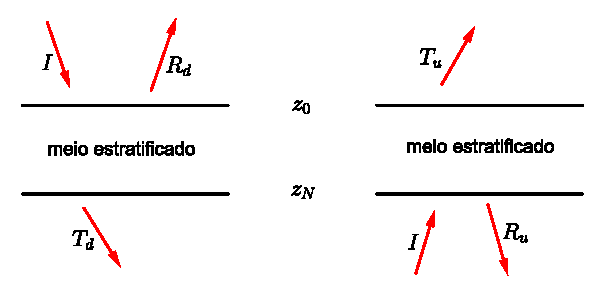
\includegraphics[scale=1.6]{ondas_ascen_descen}
\caption{\textit{Dire\c{c}\~ao e sentido de propaga\c{c}\~ao de ondas ascendentes e descendentes em camadas homog\^eneas.}}
\label{fig.ondas_ascen_descen}
\end{figure}
Vamos usar a const\^ancia da fun\c{c}\~ao dada na equa\c{c}\~ao \ref{eq.G(V,W)} para igualar seus valores calculados no topo e no fundo da pilha de camadas. Mas aqui, vamos tomar as ondas $V$ e $W$ com for\c{c}a $I$ em sentido descendente e ascendente, respectivamente.  
\begin{equation*}
\begin{bmatrix}
R_d^\top&I
\end{bmatrix}
\begin{bmatrix}
0&I\\
-I&0
\end{bmatrix}
\begin{bmatrix}
T_u\\
0
\end{bmatrix}
=
\begin{bmatrix}
0&T_d^\top
\end{bmatrix}
\begin{bmatrix}
0&I\\
-I&0
\end{bmatrix}
\begin{bmatrix}
I\\
R_u
\end{bmatrix}\,,
\end{equation*}
de onde conclu\'imos que
\begin{equation}\label{eq.T}
T_u=T_d^\top\,.
\end{equation}
Podemos ainda calcular o valor da fun\c{c}\~ao usando somente ondas descendentes $G(V,V)$. Igualando seus valores para o topo e a base da pilha de camadas, temos
\begin{equation*}
\begin{bmatrix}
R_d^\top&I
\end{bmatrix}
\begin{bmatrix}
0&I\\
-I&0
\end{bmatrix}
\begin{bmatrix}
R_d\\
0
\end{bmatrix}
=
\begin{bmatrix}
0&R_d^\top
\end{bmatrix}
\begin{bmatrix}
0&I\\
-I&0
\end{bmatrix}
\begin{bmatrix}
I\\
R_d
\end{bmatrix}\,,
\end{equation*}
de onde conclu\'imos que 
\begin{equation}\label{eq.R_d}
R_d=R_d^\top\,.
\end{equation}
Analogamente, para ondas ascendentes $G(W,W)$, temos \begin{equation}\label{eq.R_u}
R_u=R_u^\top\,.
\end{equation}
Utilizando as equa\c{c}\~oes \ref{eq.T}, \ref{eq.R_d} e \ref{eq.R_u}, podemos definir uma matriz $R$ onde as componentes representam todas as ondas refletidas e transmitidas,
\begin{equation*}
R=
\begin{bmatrix}
R_d&T_u\\
T_d&R_u
\end{bmatrix}\,,
\end{equation*}
e verificar que 
\begin{equation*}
R=R^\top\,.
\end{equation*}
A matriz $R$ est\'a relacionada \`a matriz $S$ usada em \textit{Teoria de Dispers\~ao} de ondas,
\begin{equation*}
S=
\begin{bmatrix}
T_d&R_u\\
R_d&T_u
\end{bmatrix}\,,
\end{equation*}
e a matriz $S$ relaciona, de forma linear, ondas saindo de uma pilha de camadas com ondas entrando na pilha,
\begin{equation*}
\begin{bmatrix}
\mathbf{D}(z_N)\\
\mathbf{U}(z_0)
\end{bmatrix}
=
S(z_0,z_N)\,
\begin{bmatrix}
\mathbf{D}(z_0)\\
\mathbf{U}(z_N)
\end{bmatrix}\,.
\end{equation*} 

\subsection{Rela\c{c}\~ao das Matrizes de Transmiss\~ao e Reflex\~ao com a matriz de Propaga\c{c}\~ao}

As matrizes de reflex\~ao e transmiss\~ao podem ser escritas em termos das submatrizes da matriz de propaga\c{c}\~ao, da seguinte forma:
\begin{align}\nonumber
T_u(z_0,z_N)&=Q_{11}^{-1}(z_N,z_0)\,,\\\nonumber
R_u(z_0,z_N)&=Q_{21}(z_N,z_0)\,Q_{11}^{-1}(z_N,z_0)\,,\\\label{eq.relacao_Q_R_T}
R_d(z_0,z_N)&=-Q_{11}^{-1}(z_N,z_0)\,Q_{12}(z_N,z_0)\,,\\\nonumber
T_d(z_0,z_N)&=Q_{22}(z_N,z_0)-Q_{21}(z_N,z_0)\,Q_{11}^{-1}(z_N,z_0)\,Q_{12}(z_N,z_0)\,,
\end{align}
e a matriz de propaga\c{c}\~ao \'e dada em fun\c{c}\~ao das matrizes de reflex\~ao e transmiss\~ao por
\begin{equation*}
Q(z_0,z_N)=
\begin{bmatrix}
T_u^{-1}&-T_u^{-1}R_d\\
R_uT_u^{-1}&T_d-R_uT_u^{-1}R_d
\end{bmatrix}\,.
\end{equation*}


Para o caso de camadas homog\^eneas, usando as equa\c{c}\~oes \ref{eq.Q(z,z_0)} e \ref{eq.relacao_Q_R_T}, podemos deduzir que, para matrizes de transmiss\~ao,
\begin{equation*}
T_d(z_0,z)=T_u(z_0,z)=\exp\left[\pm i\omega\,\Lambda(z-z_0)\right]\,,
\end{equation*}
e para matrizes de reflex\~ao
\begin{equation*}
R_d(z_0,z)=R_u(z_0,z)=0\,.
\end{equation*}

Vamos definir $E_{k+1}(-\pm i\omega)=\exp\left[-\pm i\omega\,\Lambda(z_{k+1}-z_k)\right]$. Assim, a matriz $S$ para uma camada homog\^enea e para interface para a pr\'oxima camada \'e dada pelo \textit{produto estrela},
\begin{align*}
S(z_{k+},z_{k+1+})&=S(z_{k+},z_{k+1-})*S(z_{k+1-},z_{k+1+})\\\\
&=
\begin{bmatrix}
E_{k+1}(-\pm i\omega)&0\\
0&E_{k+1}(-\pm i\omega)
\end{bmatrix}
*
\begin{bmatrix}
T_{d,k+1}&R_{u,k+1}\\
R_{d,k+1}&T_{u,k+1}
\end{bmatrix}\\\\
&=
\begin{bmatrix}
T_{d,k+1}E_{k+1}(-\pm i\omega)&R_{u,k+1}\\
E_{k+1}(-\pm i\omega)R_{d,k+1}E_{k+1}(-\pm i\omega)&E_{k+1}(-\pm i\omega)T_{u,k+1}
\end{bmatrix}\,.
\end{align*}